





% \section{Proofs}

% \subsection{Proof of Proposition~\ref{prop:continuous-lip}}
% \label{proof:continuous-lip}

% \begin{proof}
% Consider the time derivative of the square difference between the two flows $x_t$ and $z_t$ associated with the function $F_t$ and following the definition~\ref{def:flow}: 
% \begin{align*}
%   \frac{d}{dt} \lVert x_t-z_t\rVert_2^2 & = 2 \big\langle x_t-z_t,\frac{d}{dt}( x_t-z_t)\big\rangle\\
%     &=2 \big\langle x_t-z_t,F_{\theta_{t}}(x_{t})-F_{\theta_{t}}(z_{t})\big\rangle \\
%     &=  2 \big\langle x_t-z_t,\int_0^1\nabla_xF_{\theta_{t}}(x_{t}+s(z_t-z_t))(x_t-z_t)ds\big\rangle\textrm{, by Taylor-Lagrange formula}\\ 
%     &=  2 \int_0^1\big\langle x_t-z_t,\nabla_xF_{\theta_{t}}(x_{t}+s(z_t-z_t))(x_t-z_t)\big\rangle ds\\
%      &=  2 \int_0^1\big\langle x_t-z_t,S(\nabla_xF_{\theta_{t}}(x_{t}+s(z_t-z_t)))(x_t-z_t)\big\rangle ds
% \end{align*}
% In the last step, we used that for every skew-symmetric matrix $A$ and vector $x$, $\lVert x,Ax\rVert = 0$.
% Since $\mu_tI\preceq S(\nabla_xF_{\theta_{t}}(x_{t}+s(z_t-y_t)))\preceq  \lambda_tI$, we get
% \begin{align*}
%  2\mu_t \lVert x_t-z_t\rVert_2^2 \leq \frac{d}{dt} \lVert x_t-z_t\rVert_2^2 \leq 2\lambda_t \lVert x_t-z_t\rVert_2^2
% \end{align*}
% Then by Gronwall Lemma, we have
% \begin{align*}
%   \lVert x_0-y_0 \rVert e^{\int_0^t\mu_s ds}\leq \lVert x_t-y_t \rVert\leq \lVert x_0-y_0 \rVert e^{ \int_0^t\lambda_s ds}
% \end{align*}
% which concludes the proof.
% \end{proof}

% \subsection{Proof of Corollary~\ref{cor:conv-skew}}
% \label{proof:conv-skew}
% \begin{proof}

% For all $t,x$, we have $F_t(x) = -\nabla_x f_{t}(x)+A_t x$ ~ so~
% $\nabla_x F_t(x) = -\nabla_x^2 f_{t}(x)+A_t$. Then $S(\nabla_x F_t(x)) =-\nabla_x^2 f_{t}(x)$. Since $f$ is convex, we have $\nabla_x^2 f_{t}(x)\succeq 0$. So by application of Proposition~\ref{prop:continuous-lip}, we deduce $\lVert x_t-y_t \rVert\leq \lVert x_0-y_0 \rVert$ for all trajectories starting from $x_0$ and $y_0$.
% \end{proof}

% \subsection{Proof of Proposition~\ref{prop:discrete_convex_potentials}}
% \label{proof:discrete_convex_potentials}
% \begin{proof}
% With $c_t = \lVert x_t -z_t\rVert_2^2$, we can write:
% \begin{align*}
%    c_{t+\frac12} - c_t = &-2 h_t \big\langle x_t - z_t, \nabla_xF_{\theta_{t}}(x_t) - \nabla_xF_{\theta_{t}}(z_t)  \big\rangle+ h_t^2 \lVert \nabla_xF_{\theta_{t}}(z_t) - \nabla_xF_{\theta_{t}}(z_t)\rVert_2^2
% \end{align*}
% This equality allows us to derive the equivalence between  $c_{t+1} \leq c_t$ and: 
% \begin{align*}
%    \frac{h_t}{2}
%    \lVert  \nabla F_{\theta_{t}}(x_t) - \nabla F_{\theta_{t}}(z_t)\rVert_2^2
%    \leq
%    \langle x_t -z_t, \nabla F_{\theta_{t}}(z_t) - \nabla F_{\theta_{t}}(z_t) \rangle 
% \end{align*}
% Moreover, assuming that $F_{\theta_t}$ being  that:
% \begin{align*}
%    \frac{1}{L_t} &\lVert \nabla_xF_{\theta_{t}}(x_t) - \nabla_xF_{\theta_{t}}(z_t)\rVert_2^2 
%    \leq\big\langle x_t -z_t, \nabla_xF_{\theta_{t}}(x_t) - \nabla_xF_{\theta_{t}}(z_t) \big\rangle
% \end{align*}
% We can see with this last inequality that if we enforce  $h_t \leq \frac{2}{L_t}$, we get $c_{t+\frac12} \leq c_t$ which concludes the proof.
% \end{proof}


% \section{Additional Results}

% % \subsection{Functions whose gradient is skew-symmetric everywhere}
% % \label{sup:skew}
% Let $F:=(F_1,\dots,F_d):\RR^d\to\RR^d$ be a twice differentiable function such that $\nabla F(x)$ is skew-symmetric for all $x\in\RR^d$. Then we have for all $i,j,k$:
% \begin{align*}
%     \partial_i\partial_j F_k =  -\partial_i\partial_k F_j =-\partial_k\partial_i F_j = \partial_k\partial_j F_i = \partial_j\partial_k F_i = -\partial_j\partial_i F_k = -\partial_i\partial_j F_k
% \end{align*}
% So we have $\partial_i\partial_j F_k =0$ and then $F$ is linear: there exists a skew-symmetric matrix $A$ such that $F(x)=Ax$ 


% \subsection{Implicit discrete convex potential flows}
% \label{sup:implicit}

% Let us define the implicit update $x_{t+\frac12} = x_{t}-\nabla_xf_{t}(x_{t+\frac12})$. Let us remark that $x_{t+\frac12}$ is uniquely defined as:
% \begin{align*}
%  x_{t+\frac12} =\argminB_{x\in\RR^d} \frac 12\lVert x-x_t\rVert^2+ f_t(x)  
% \end{align*}
% We recognized here the proximal operator of $f_t$ that is uniquely defined since $f_t$ is convex. Moreover we have for two trajectories $x_t$ and $z_t$:
% \begin{align*}
%    \lVert x_t-z_t\rVert^2_2& =  \lVert x_{t+\frac12}-z_{t+\frac12} +\nabla_xf_{t}(x_{t+\frac12})-\nabla_xf_{t}(z_{t+\frac12}) \rVert^2_2 \\
%    &=  \lVert x_{t+\frac12}-z_{t+\frac12}\rVert^2 + 2\langle x_t-z_t,\nabla_xf_{t}(x_{t+\frac12})-\nabla_xf_{t}(z_{t+\frac12})\rangle +\lVert\nabla_xf_{t}(x_{t+\frac12})-\nabla_xf_{t}(z_{t+\frac12}) \rVert^2_2 \\
%    &\geq  \lVert x_{t+\frac12}-z_{t+\frac12}\rVert^2 
% \end{align*}
% where the last inequality is deduced from the convexity of $f_t$. So, without any further assumption on $f_t$, the discretized implicit convex potential flow is $1$-Lipschitz.

% To compute such a layer, one could solve the proximal operator strongly convex-minimization optimization problem. This strategy is not computationally efficient and not scalable. 




% \subsection{Expressivity of discretized convex potential flows}
% \label{app:express}
% Let us define $\mathcal{S}_1(\RR^{d\times d})$ the space of real symmetric matrices with singular values bounded by $1$. Let us also define $\mathcal{M}_1(\RR^{d\times d})$ the space of real matrices with singular values bounded by $1$ in absolute value.
% Let $\mathcal{P}(\RR^{d\times d})=\{A\in\RR^{d\times d}|\exists n\in \mathbb{N},S_1,\dots,S_n\in \mathcal{S}_1(\RR^d\times d)\text{ s.t. } A = S_1\dots S_n\}$. Then one can prove\footnote{A proof and justification of this result can be found here: \url{https://mathoverflow.net/questions/60174/factorization-of-a-real-matrix-into-hermitian-x-hermitian-is-it-stable}} that $\mathcal{P}(\RR^{d\times d}) \neq \mathcal{M}_1(\RR^{d\times d})$. Thus there exists $A\in\mathcal{M}_1(\RR^{d\times d})$ such that for all matrices $n$, for all matrices $S_1,\dots,S_n\in\mathcal{S}_1(\RR^{d\times d})$ such that $M\neq S_1,\dots,S_n$. 

% Applied to the expressivity of discretized convex potential flows, the previous result means that there exists a $1$-Lipschitz linear function that cannot be approximated as a discretized flow of any depth of convex linear $1$-smooth potential flows as in Proposition~\ref{prop:discrete_convex_potentials}. Indeed such a flow would write: $x\mapsto\prod_i(1-2S_i)x$ where $S_i$ are symmetric matrices whose eigenvalues are in $[0,1]$, in other words such transformations are exactly described by $x\mapsto Mx$  for some $M\in\mathcal{P}(\RR^{d\times d})$.




\section{Additional experiments}
\label{app:xp-supp}

\subsection{Training stability: scaling up to $1000$ layers}

\begin{figure}[h]
    \centering
    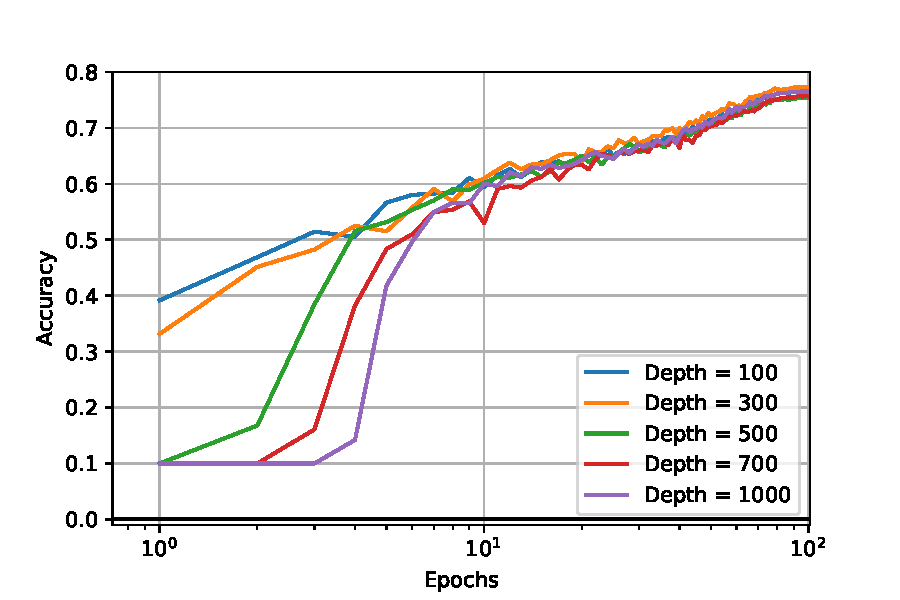
\includegraphics[width=0.5\textwidth]{sections/4_certification/images/final_cifar10_veryverydeep.pdf}
    \caption{Standard test accuracy in function of the number of epochs (log-scale) for various depths for our neural networks ($100,300,500,700,1000$).}
    \label{fig:verydeep}
\end{figure}

While the Residual Network architecture limits, by design, gradient vanishing issues, it still suffers from exploding gradients in many cases~\citep{hayou2021stable}.
To prevent such scenarii, batch normalization layers~\citep{ioffe2015batch} are used in most Residual Networks to stabilize the training.

Recently, several works~\citep{miyato2018spectral,farnia2018generalizable} have proposed to normalize the linear transformation of each layer by their spectral norm.
Such a method would limit exploding gradients but would again suffer from gradient vanishing issues.
Indeed, spectral normalization might be too restrictive: dividing by the spectral norm can make other singular values vanishingly
small.
While more computationally expensive (spectral normalization can be done with $1$ Power Method iteration), orthogonal projections prevent both exploding and vanishing issues. 

On the contrary the architecture proposed in this paper has the advantage to naturally control the gradient norm of the output with respect to a given layer.
Therefore, our architecture can get the best of both worlds: limiting exploding and vanishing issues while maintaining scalability. 
To demonstrate the scalability of our approach, we experiment the ability to scale our architecture to very high depth (up to 1000 layers) without any additional normalization/regularization tricks, such as Dropout~\citep{srivastava2014dropout}, Batch Normalization~\citep{ioffe2015batch} or gradient clipping~\citep{pascanu2013difficulty}.
With the work done by~\cite{xiao2018dynamical}, which leverage Dynamical Isometry and a Mean Field Theory to train a $10000$ layers neural network, we believe, to the best of our knowledge, to be the second to perform such training. 
For sake of computation efficiency, we limit this experiment to architecture with $30$ feature maps.
We report the accuracy in terms of epochs for our architecture in Figure~\ref{fig:verydeep} for a varying number of convolutional layers.
It is worth noting that for the deepest networks, it may take a few epochs before the start of convergence.
As \cite{xiao2018dynamical}, we remark there is no gain in using very deep architecture for this task.


\subsection{Relaxing linear layers}

\begin{center}
\begin{tabular}{lrrr}
\toprule
  & \multicolumn{1}{c}{\textbf{h = 1.0}} & \multicolumn{1}{c}{\textbf{h = 0.1}} & \multicolumn{1}{c}{\textbf{h = 0.01}} \\
\midrule
\textbf{Clean} & 85.10 & 82.23 & 78.53 \\
\textbf{PGD ($\varepsilon = 36/255$}) & 61.45 & 62.99 & 60.98 \\
\bottomrule
\end{tabular}%
\end{center}
The table above shows the result of the relaxed training of our StableBlock architecture, i.e. we fixed the step $h_t$ in the discretized convex potential flow of Proposition~\ref{prop:discrete_convex_potentials}.
Increasing the constant $h$ allows for an important improvement  in the clean accuracy, but we loose in robust empirical accuracy.
While computing the certified accuracy is not possible in this case due to the unknown value of the Lipschitz constant, we can still notice that the training of the network are still stable without normalization tricks, and offer a non-negligible level of robustness. 





\subsection{Effect of Batch Size in Training}


\begin{table*}[h]
  \centering
  \sisetup{%
    table-align-uncertainty=true,
    separate-uncertainty=true,
    detect-weight=true,
    detect-inline-weight=math
  }
  \begin{tabular}
  {
    l
    S[table-format=2.2]
    S[table-format=2.2]
    S[table-format=2.2]
    S[table-format=2.2]
    S[table-format=2.2]
    S[table-format=2.2]
  }
  \toprule
  &\multicolumn{1}{c}{\textbf{Batch size }}& \multicolumn{1}{c}{\textbf{Clean Accuracy}} & \multicolumn{3}{c}{\textbf{Provable Accuracy ($\varepsilon $)}} &  \multicolumn{1}{c}{\textbf{Time per epoch (s)}} 
    \\
    \cmidrule{4-6}
    & \multicolumn{1}{c}{ } & \multicolumn{1}{c}{ } &\multicolumn{1}{c}{36/255} & \multicolumn{1}{c}{72/255} &  \multicolumn{1}{c}{108/255} & \multicolumn{1}{c}{\textbf{}} 
    \\
  \midrule
    \multirow{3}{*}{\textbf{CPL-S}} & 64 & 76.5& 62.9 & 47.3 & 32.0 & 48 \\
                                    & 128 & 76.1 & 62.8 & 47.1 & 32.3  & 31 \\
                                    & 256 & 75.6 & 62.3 & 46.9 & 32.2 & 22 \\
    \midrule
 \multirow{3}{*}{\textbf{CPL-M}} & 64 & 77.4 & 63.6 & 47.4 & 32.1  & 77 \\
                                    & 128 & 77.2 &63.5 & 47.5 & 32.1 & 50 \\
                                    & 256 & 76.8 & 63.2 & 47.4 & 32.4& 40 \\
    \midrule

 \multirow{3}{*}{\textbf{CPL-L}} & 64 & 78.4 & 64.2 & 47.8 & 32.2  & 162 \\
                                    & 128 & 78.2 & 64.3 & 47.9 & 32.5 & 109 \\
                                    & 256 & 77.6 & 63.9 & 48.1 & 32.7& 93 \\
  \midrule
 \multirow{3}{*}{\textbf{CPL-XL}} & 64 & 78.9 & 64.2 & 47.2 & 31.2  & 271 \\
                                    & 128 & 78.9 & 64.2 & 47.5 & 31.8 & 198 \\
                                    & 256 &78.5 & 64.4 & 47.8 & 32.4& 163 \\

  \bottomrule
  \end{tabular}%
  \caption{Results on the CIFAR10 dataset on standard and  provably certifiable accuracies for different values of perturbations $\varepsilon$ on CPL (ours) models with various batch sizes. The average time per epoch in seconds is also reported in the last column. All the reported networks use Last Layer Normalization.}
  \label{table:c10-comp-bs}%
\end{table*}%



\begin{table*}[h]
  \centering
  \sisetup{%
    table-align-uncertainty=true,
    separate-uncertainty=true,
    detect-weight=true,
    detect-inline-weight=math
  }
  \begin{tabular}
  {
    l
    S[table-format=2.2]
    S[table-format=2.2]
    S[table-format=2.2]
    S[table-format=2.2]
    S[table-format=2.2]
    S[table-format=2.2]
  }
  \toprule
  &\multicolumn{1}{c}{\textbf{Batch size }}& \multicolumn{1}{c}{\textbf{Clean Acc.}} & \multicolumn{3}{c}{\textbf{Provable Acc. ($\varepsilon $)}} &  \multicolumn{1}{c}{\textbf{Time per epoch (s)}} 
    \\
    \cmidrule{4-6}
    & \multicolumn{1}{c}{ } & \multicolumn{1}{c}{ } &\multicolumn{1}{c}{36/255} & \multicolumn{1}{c}{72/255} &  \multicolumn{1}{c}{108/255} & \multicolumn{1}{c}{\textbf{}} 
    \\
  \midrule
  \multirow{3}{*}{\textbf{CPL-S}} & 64 & 45,6 & 30,8 & 19,3 & 11,2 & 47 \\
                                    & 128 & 44,9 & 30,7 & 19,2 & 11,0 & 31\\
                                    & 256 & 44,0 & 29,9 & 19,1 & 10,9 & 23\\
  \midrule
  \multirow{3}{*}{\textbf{CPL-M}} & 64 & 46.6 & 31,6 & 19,6 & 11,6 & 78 \\
                                    & 128 & 46.3 & 31,1 & 19,7 & 11,5 & 55 \\
                                    & 256 & 45.6 & 31,1 & 19,3 & 11,3 & 41 \\

  \midrule

  \multirow{3}{*}{\textbf{CPL-L}} & 64 & 48.1 & 32,7 & 20,3 & 11,7 & 163 \\ 
                                    & 128 & 47,4 & 32,3 & 20,0 & 11,8 & 116 \\ 
                                    & 256 & 46,8 & 31,8 & 20,1 & 11,7 & 95 \\ 
  \midrule
  \multirow{3}{*}{\textbf{CPL-XL}} & 64 & 49,0 & 33,7 & 21,1 & 12,0 & 293 \\
                                    & 128 & 48,0 & 33,7 & 21,0 & 12,1 & 209 \\
                                    & 256 &47,8 & 33,4 & 20,9 & 12,6 & 164 \\

  \bottomrule
  \end{tabular}%
  \caption{Results on the CIFAR100 dataset on standard and  provably certifiable accuracies for different values of perturbations $\varepsilon$ on CPL (ours) models with various batch sizes. The average time per epoch in seconds is also reported in the last column. All the reported networks use Last Layer Normalization.}
  \label{table:c100-comp-bs}%
\end{table*}%

In Tables~\ref{table:c10-comp-bs} and~\ref{table:c100-comp-bs}, we tried three different batch sizes (64, 128 and 256) for training our networks on CIFAR10 and CIFAR100 datasets, we remark a gain in standard accuracy in reducing the batch size for all settings. As the perturbation becomes larger, the gain in accuracy is reduced and can even in some cases we may loose some points in robustness.

\subsection{Effect of the Margin Parameter}

\begin{figure}[h]
    \centering
    \begin{tabular}{cc}
    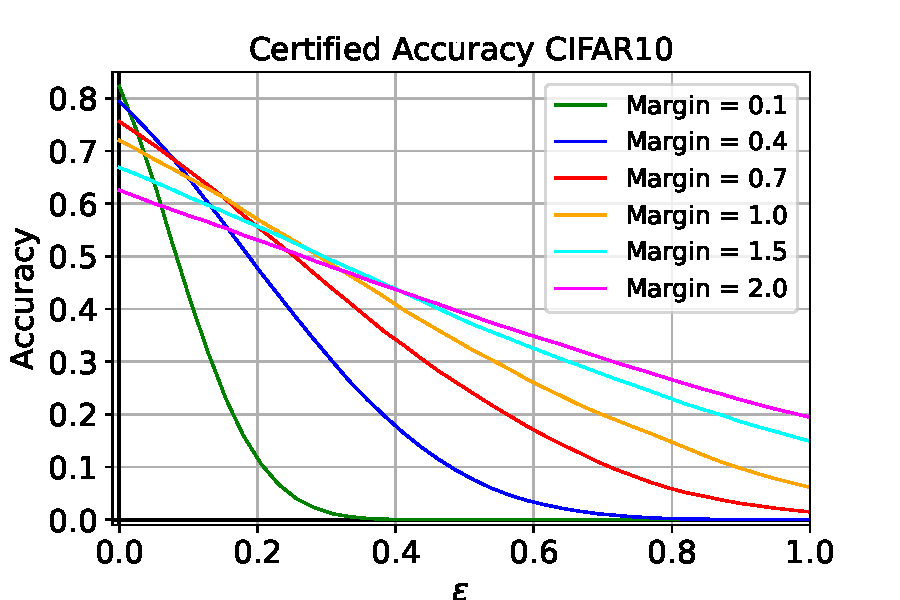
\includegraphics[width=0.49\textwidth]{sections/4_certification/images/cert_acc_margin_eps_c10.pdf}&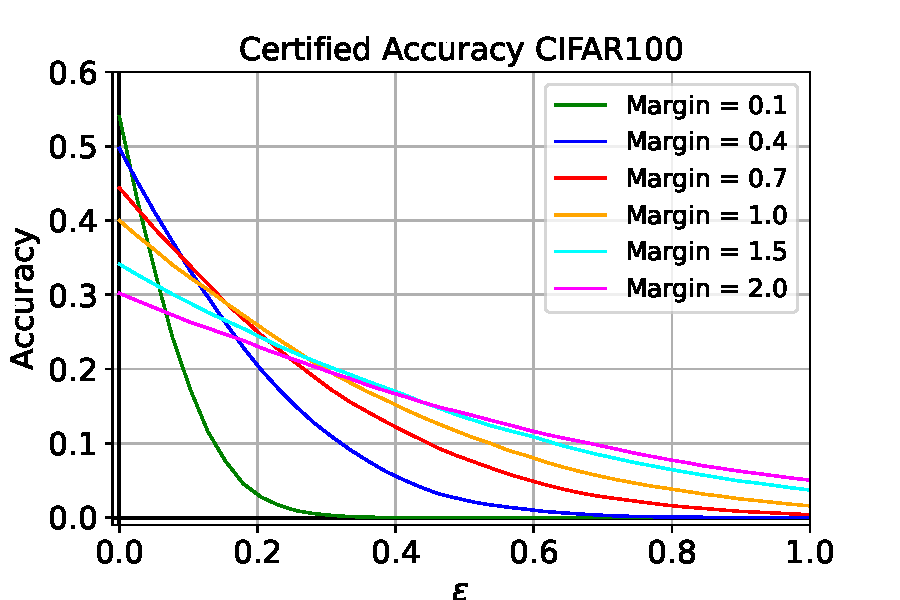
\includegraphics[width=0.49\textwidth]{sections/4_certification/images/cert_acc_margin_eps_c100.pdf}
    \end{tabular}
    \caption{Certifiably robust accuracy in function of the perturbation $\varepsilon$ for our CPL-S  network with different margin parameters on CIFAR10 and CIFAR100 datasets.}
    \label{fig:cert-acc-margin}
\end{figure}


\begin{figure}[h]
    \centering
    \begin{tabular}{cc}
    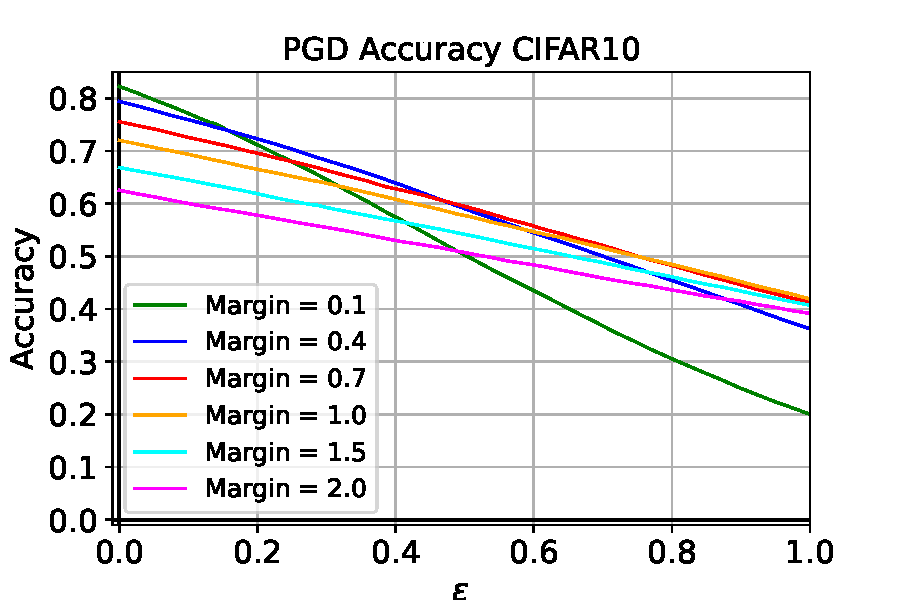
\includegraphics[width=0.49\textwidth]{sections/4_certification/images/pgd_acc_margin_eps_c10.pdf}&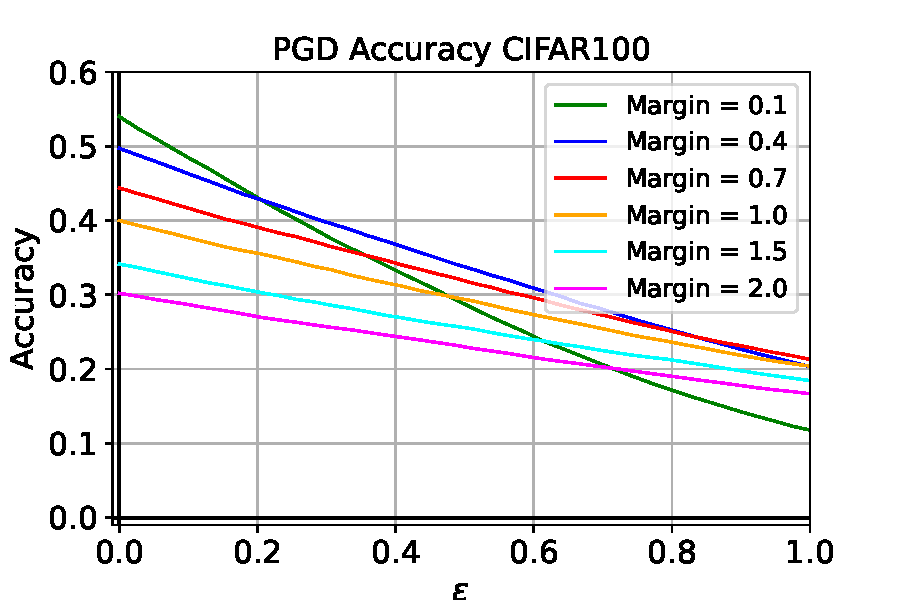
\includegraphics[width=0.49\textwidth]{sections/4_certification/images/pgd_acc_margin_eps_c100.pdf}
    \end{tabular}
    \caption{Certifiably robust accuracy in function of the perturbation $\varepsilon$ for our CPL-S  network with different margin parameters on CIFAR10 and CIFAR100 datasets.}
    \label{fig:pgd-acc-margin}
\end{figure}

In these experiments we varied the margin parameter in the margin loss in Figures~\ref{fig:cert-acc-margin} and~\ref{fig:pgd-acc-margin}. It clearly exhibits a tradeoff between standard and robust accuracy. When the margin is large, the standard accuracy is low, but the level of robustness remain high even for ``large'' perturbations. On the opposite, when the margin is small, we get a high standard accuracy but we are unable to keep a good robustness level as the perturbation increases. It is verified both on certified and empirical robustness.
